%!TEX root = ../NCVC7.tex
\mysection{等高線のNCデータを生成}

\subsection{等高線パスの生成}
 等高線のデータを生成するには,切削対象となるNURBS曲面を1つ選択する必要があります.
マウスの左クリックで選択してください.

 NURBS曲面が選択されていると,\menu{ファイル>NCデータの生成>等高線パスの生成}(\keys{F3})のメニューが有効になります.
図~\ref{fig:ncvc31} のダイアログから適当な値を設定してください.

\begin{figure}[H]
\centering
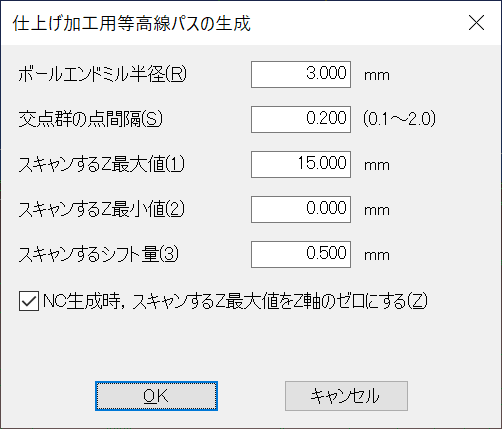
\includegraphics{No3/fig/fig31.png}
\caption{等高線パスの設定}
\label{fig:ncvc31}
\end{figure}

 図~\ref{fig:ncvc31} で \keys{OK} を押すと,図~\ref{fig:ncvc32} のように等高線パスが表示されます.
この等高線はNURBS曲面上に点群がプロットされます.
裏面を見ると 図~\ref{fig:ncvc33} のように点群が貫通して見えますが気にしないでください
\footnote{ポリゴンオフセットという手法で面を少しだけずらして描画しています.こうしないと表面であっても「zファイティング」と言われる不自然なレンダリング結果になります.スキャニングパスで曲面オフセットをゼロにしたときも同様です.}.

\begin{figure}[H]
\centering
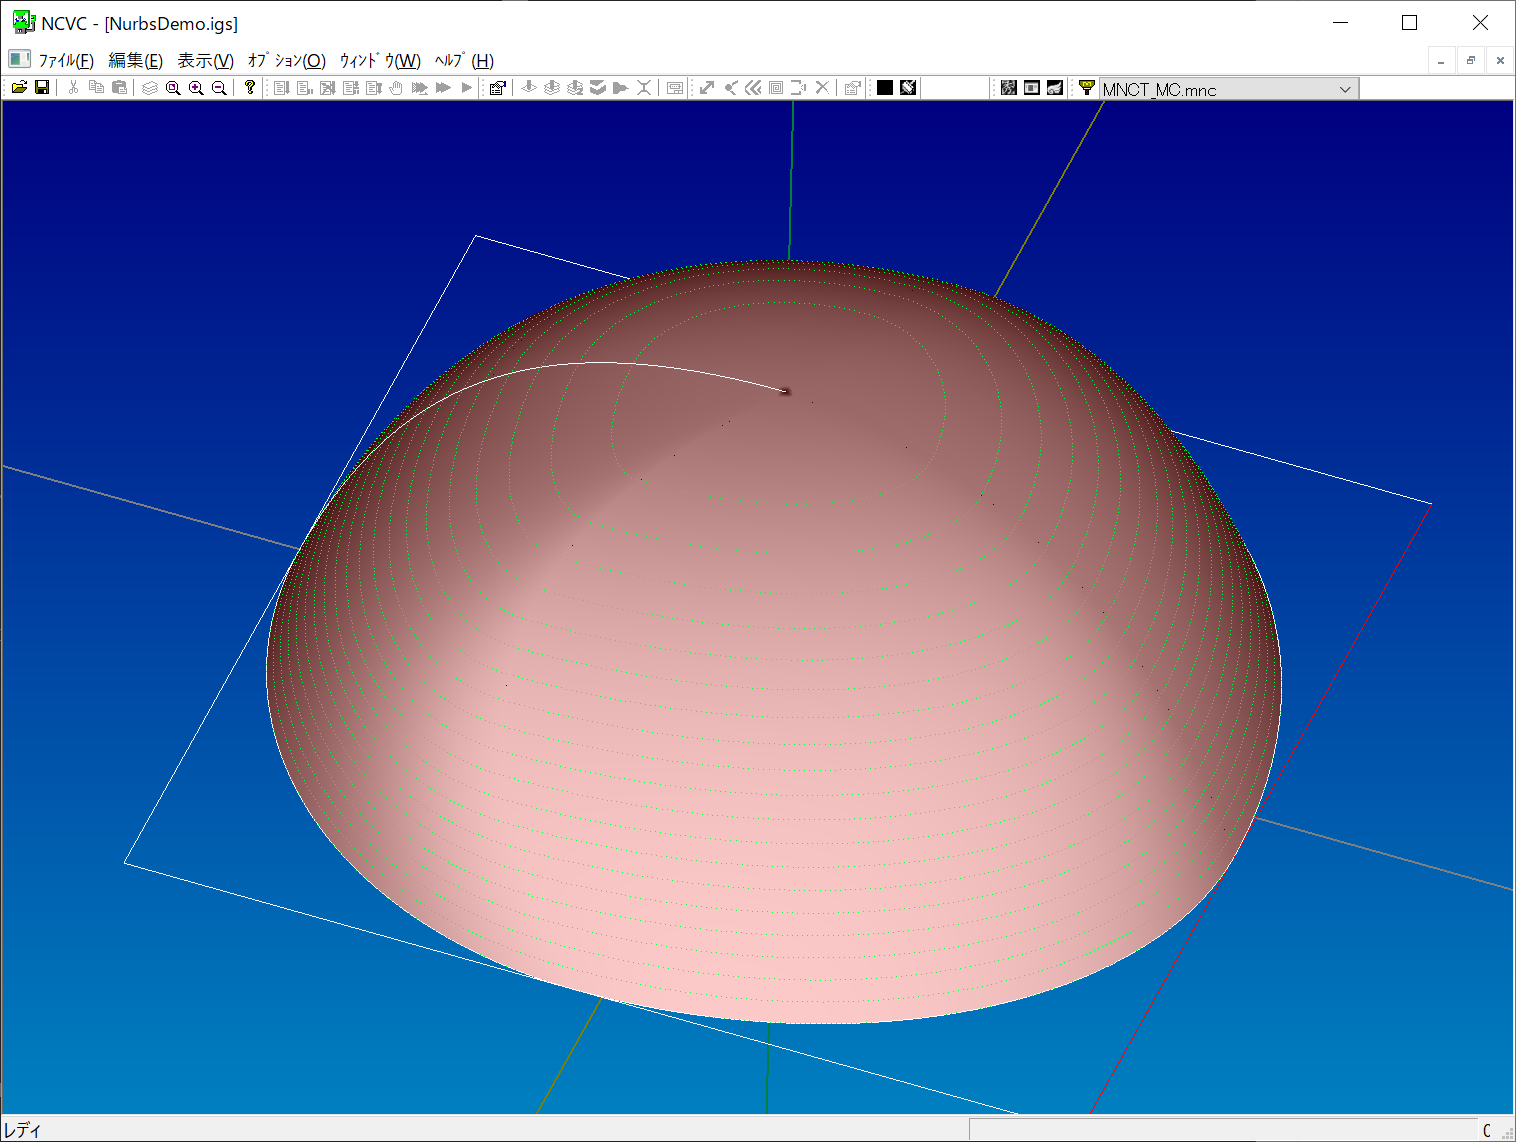
\includegraphics[scale=0.5]{No3/fig/fig32.png}
\caption{等高線パスの表示}
\label{fig:ncvc32}
\end{figure}

\begin{figure}[H]
\centering
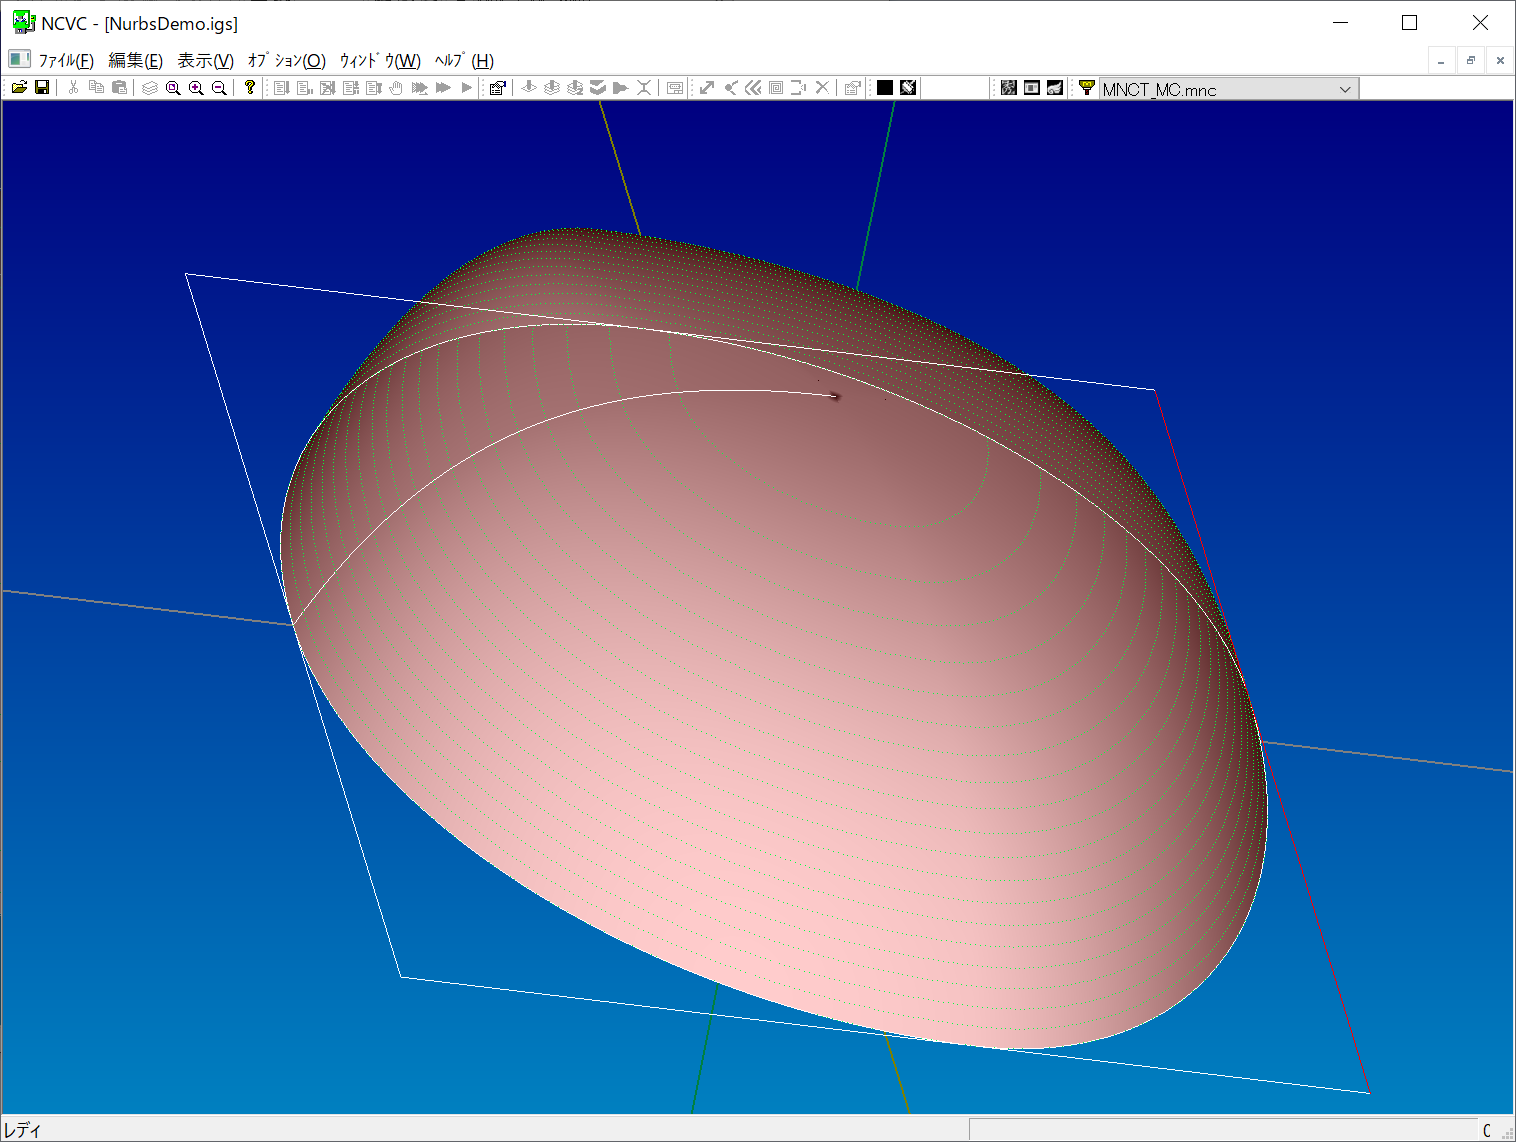
\includegraphics[scale=0.5]{No3/fig/fig33.png}
\caption{裏面のようす}
\label{fig:ncvc33}
\end{figure}

\newpage
\subsection{NCデータの出力とシミュレーション結果}
 スキャニングパスと同じように \menu{ファイル>NCデータの生成>3D切削データの出力}(\keys{F7})のメニューから出力できます.
出力ファイル名にはデフォルトで \_Contour というサフィックス(接尾語)が付けられます(図~\ref{fig:ncvc34}).
切削条件は 図~\ref{fig:ncvc27} と同じなので省略します.

\begin{figure}[H]
\centering
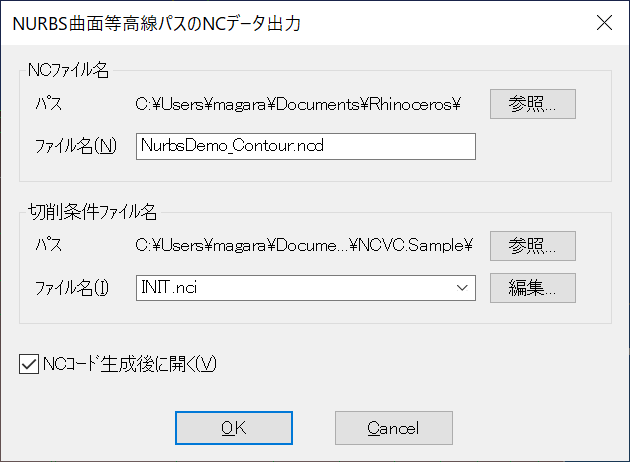
\includegraphics[scale=0.7]{No3/fig/fig34.png}
\caption{等高線用NCデータの出力設定}
\label{fig:ncvc34}
\end{figure}

 用途や形状に応じてスキャニングパスと使い分けてください.
必要なら手作業で2つのパスを連結しても良いかもしれません.

\begin{figure}[H]
\centering
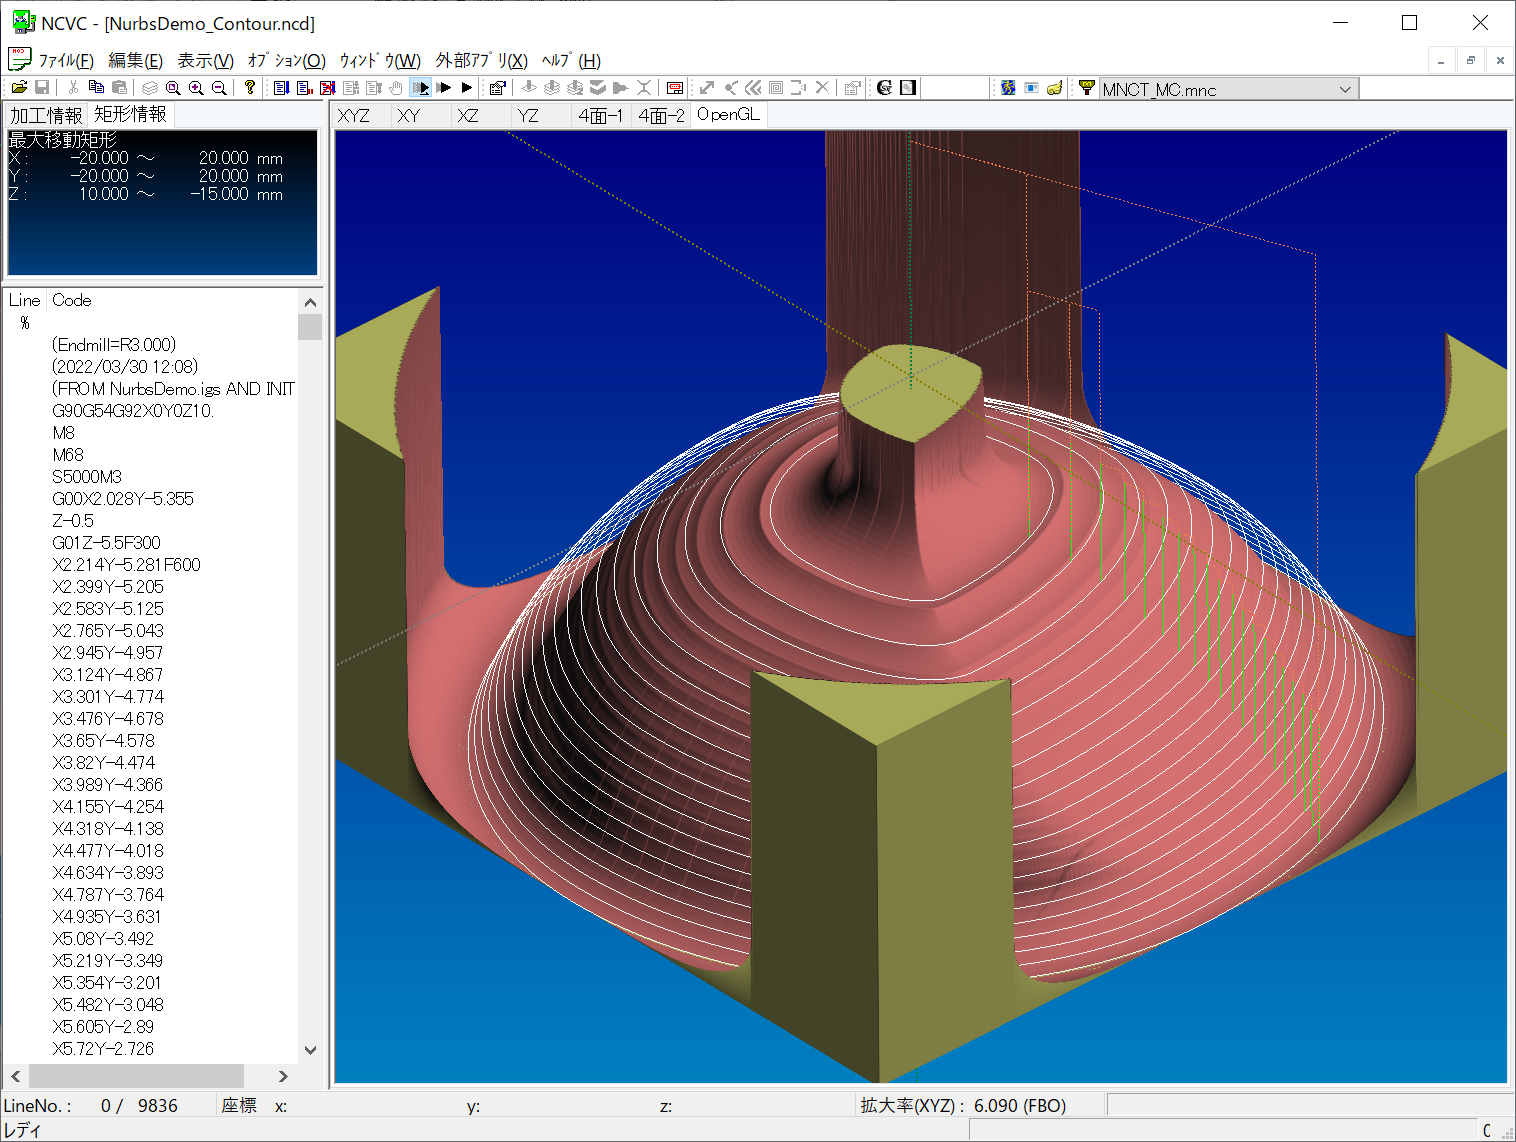
\includegraphics[scale=0.5]{No3/fig/fig35.png}
\caption{等高線NCデータのシミュレーション結果}
\label{fig:ncvc35}
\end{figure}

\newpage
\begin{itembox}[l]{ここまでの【まとめ】}
(1) IGESデータ
\begin{itemize}
\item NURBSの曲線と曲面のみ
\item NCVCが落ちる場合もある
\item 読めない場合はIGESタイプを変更
\end{itemize}
(2) スキャニングパス
\begin{itemize}
\item NURBS曲面とガイドとなるNURBS曲線を選択
\item \keys{F2}$\rightarrow$\keys{F7} でシミュレーション確認
\item ダメなら \keys{F6} $\rightarrow$ガイド曲線や設定を変える$\rightarrow$\keys{F2}$\rightarrow$\keys{F7}
\item 曲面オフセットをゼロにすると仕上げパスになる
\end{itemize}
(2) 等高線
\begin{itemize}
\item NURBS曲面を選択
\item \keys{F3}$\rightarrow$\keys{F7} でシミュレーション確認
\item ダメなら \keys{F6} $\rightarrow$設定を変える$\rightarrow$ \keys{F3}$\rightarrow$\keys{F7}
\item 用途や形状によってスキャニングパスと等高線パスを使い分ける
\end{itemize}
\end{itembox}
